\documentclass[../main/main.tex]{subfiles}

\newdate{date}{16}{10}{2020}


\begin{document}

\marginpar{ \textbf{Lecture 7.} \\  \displaydate{date}. \\ Compiled:  \today.}

To summarize what we have seen last lecture: it holds for most real networks that the average path length scales as:
\begin{equation*}
  \expval{l} \approx \ln{N}
\end{equation*}
the logarithm of the number of nodes in the network, not just with the number of nodes. Or in some cases as \( \expval{l} \approx \ln(\ln(N))  \).
But how is it possible? A paper which explains it is “Collective dynamics of small world networks” by Watts and Strogatz. Their idea is what is called the \textbf{Watts and Strogatz model}.

\begin{figure}[h!]
\centering
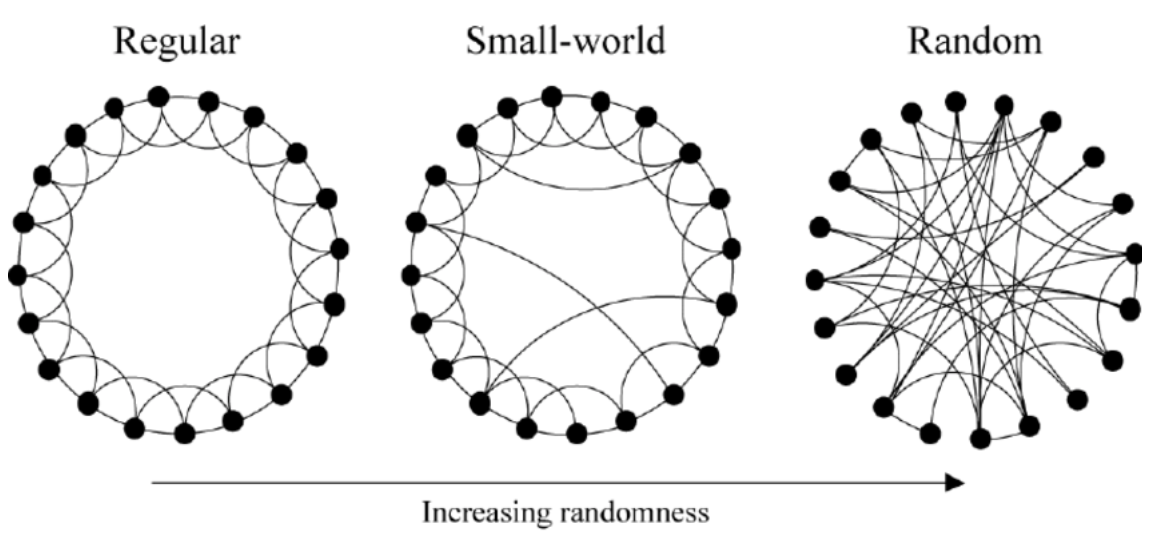
\includegraphics[width=0.7\textwidth]{../lessons/image/06/1.png}
\caption{\label{fig:06_1} Idea of Watts and Strogatz model.}
\end{figure}


Let us focus on the first regular ring in Fig. \ref{fig:06_1}, in which we have that each node is connected with its two nearest neighbours in both sides. The structure as we can see is totally regular. If we want to measure the \textbf{longest distance} that we can find in the network:
\begin{equation*}
  \expval{l^{circle}} \sim \frac{N}{4 m}
\end{equation*}
But what actually happens if we rewire only a single link? We therefore want to connect it with another random node in the network as in the picture in the middle "small-world" in Fig. \ref{fig:06_1}. It can be seen that, by doing a single rewiring, the size of the system reduces in an incredible way. On the other hand, if we extend this argument and choose a probability $p$ for rewiring (i.e. we increase randomness), what happens is that every time we rewire a connection, the average distance is reduced by a factor 2. Repeating this process several times, we observe a \textbf{logarithmic scaling}. Finally, the random network we obtain scales as:
\begin{equation*}
  \expval{l} \sim \log{N}
\end{equation*}
And it is represented by the random circle in Fig. \ref{fig:06_1}.

\section{Degree distribution over networks}
Now the question is how degrees are distributed for different type of networks.\\
Let us consider a \textbf{small network}, its degree distribution will be really resembling to the plot on the left of Fig. \ref{fig:06_2}. However, now we want to understand how this quantity distributes in \textbf{real networks}. In order to build a real network, the first assumption that we can make is building the connections \textit{at random}, so with a probability $p$. Consequently the degree distribution is one of the kind as in the right of Fig. \ref{fig:06_2}.

\begin{figure}[h!]
\begin{minipage}[c]{0.5\linewidth}
\centering
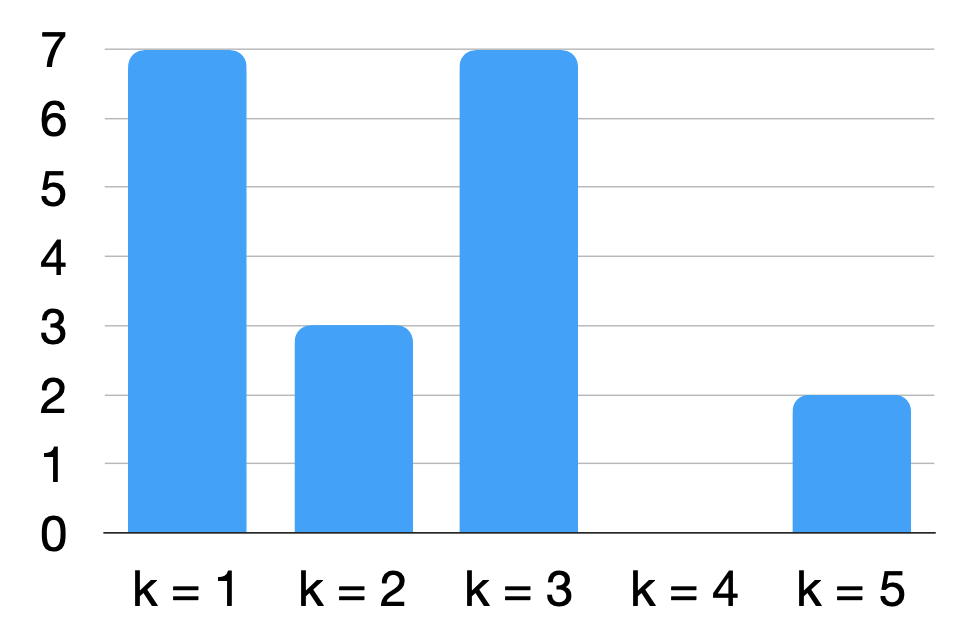
\includegraphics[width=0.8\textwidth]{../lessons/image/06/2.png}
\end{minipage}
\begin{minipage}[]{0.5\linewidth}
\centering
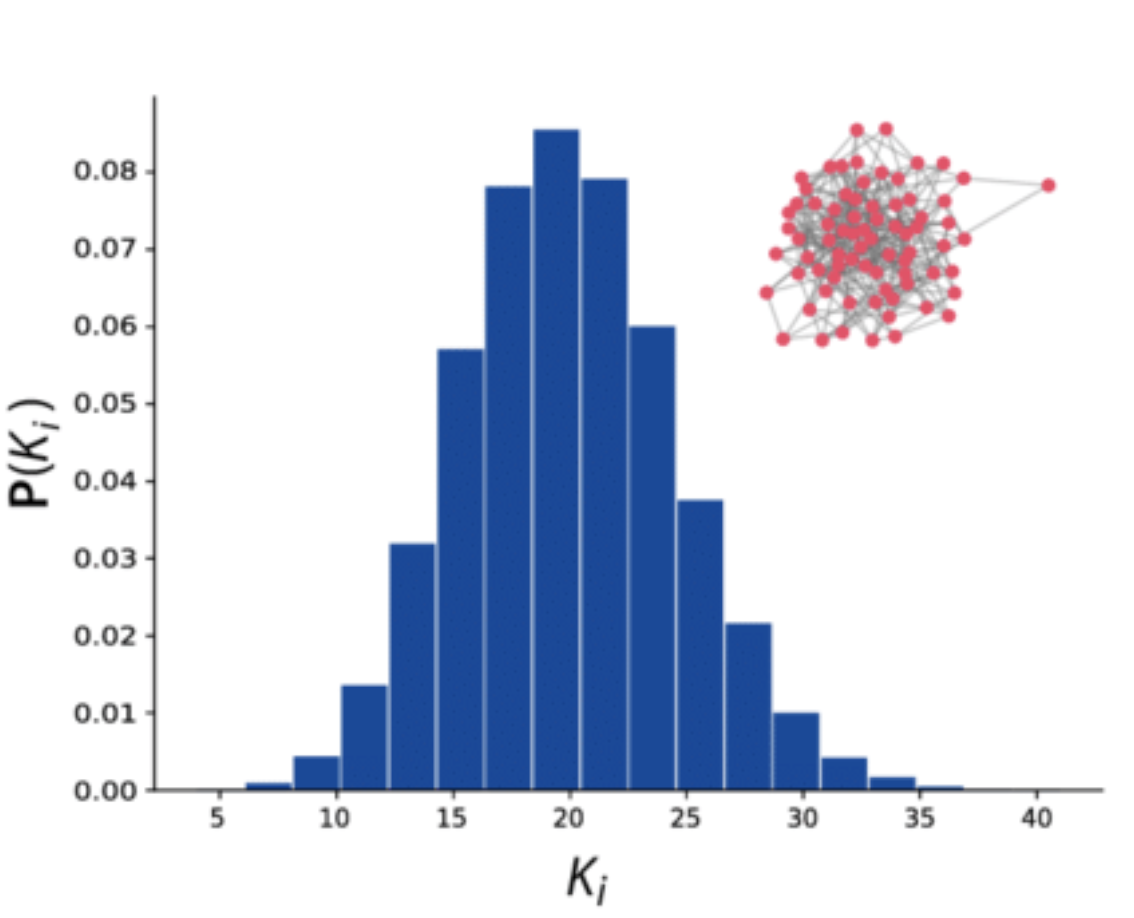
\includegraphics[width=0.8\textwidth]{../lessons/image/06/3.png}
\end{minipage}
\caption{\label{fig:06_2} \textbf{Left:} degree distribution in a small network. \textbf{Right:} degree distribution in a network with random connections. }
\end{figure}

\subsection{Erdös and Rényi Model: random graphs}
Let us consider the Erdös and Rényi model which represents the evolution of a graph where links between nodes are drawn at random, according to a predefined probability $p$. Before 1959 (the year of the publication of Erdös and Rényi's paper) people were actually assuming that connections were regular, so no randomness at all. However, since randomness in real world is a deal, thanks to E.R. random connections were taken into account for the first time.\\
In particular, the algorithm for creating such a network is:
\begin{itemize}
\item create an empty graph with $N$ nodes;
\item connect each possible couple of nodes with probability $p$;
\item avoid self-loops and multiple edges.
\end{itemize}
What are the \textbf{properties} of this graph?
Let us consider a graph \( G(N,p) \), where \( N \) are the \textbf{number of nodes} and \( p \) is the \textbf{probability of link}.
If links are drawn at random with probability $p$, the probability $p_k$ that a node has $k$ neighbors is given by a binomial distribution:
\begin{equation}
  p_k = \binom{N-1}{k} p^k (1-p)^{N-1-k}
\end{equation}
The \textbf{average} and \textbf{variance} of such a distribution are:
\begin{equation}
  \expval{k} = p(N-1), \qquad \sigma _k^2 = p(1-p)(N-1)
\end{equation}
As we can see, the average and the variance scales in the same way with the size of the network (i.e. linearly!).\\
The problem of this distribution is that it is difficult to be dealt with analytically, specially as \( N \) increases, indeed:
\begin{equation*}
  \frac{\sigma _k}{\expval{k} } = \sqrt{\frac{1-p}{p(N-1)}} \overset{N \rightarrow \infty }{\longrightarrow } 0
\end{equation*}
which becomes narrower as \( N \) becomes larger, therefore some sort of \textbf{approximation} needs to be introduced.\\

Fortunately, since for sparse networks we have \( k \ll N \), the binomial \( (N,p) \) distribution can be approximated by a \textbf{Poisson distribution} with parameter \( \lambda = p N \). Indeed, given that  \( \expval{k} = p(N-1)  \), if we have \( k \ll N \) then it implies that \( p \ll N \). Hence we can write the following:
\begin{equation*}
  (1-p)^{N-1-k} \approx e^{(N-1-k) \log (1- \expval{k}/(N-1) )} \overset{N \rightarrow \infty }{\longrightarrow } e^{- \expval{k} }
\end{equation*}
and
\begin{equation*}
  \binom{N-1}{k} \approx \frac{(N-1)^k}{k!}
\end{equation*}
Obtaining the \textbf{Poisson distribution} we were looking for:
\begin{equation}
  p_k = e^{- \expval{k} } \frac{\expval{k} }{k!}
\end{equation}
As before, the average and the variance scale exactly in the same way with the size of the network ($\sim \lambda = Np$). This actually tells us that \textbf{all} the \textbf{nodes are} more or less \textbf{the same}. Indeed when we observe a bounded variance, it means that all the nodes more or less have the same degree.\\
In particular, as $p$ increases the graph undergoes a \textbf{transition} from disconnected to fully connected one:
\begin{itemize}
\item if \( N p < 1 \), the graph will almost surely have no connected components of size larger than \( O(\log(N)) \);
\item if \( N p = 1 \), the graph will almost surely have a giant component of size \( O(N^{2/3}) \);
\item if \( N p \rightarrow c > 1 \), the graph will almost surely have a giant component comprising a large fraction of the nodes;
\item if \( p < \frac{(1- \varepsilon )\ln N}{N} \), the graph will almost surely contain isolated vertices;
\item if \( p > \frac{(1- \varepsilon )\ln N}{N} \),  the graph will almost surely be connected.
\end{itemize}

\begin{figure}[h!]
\centering
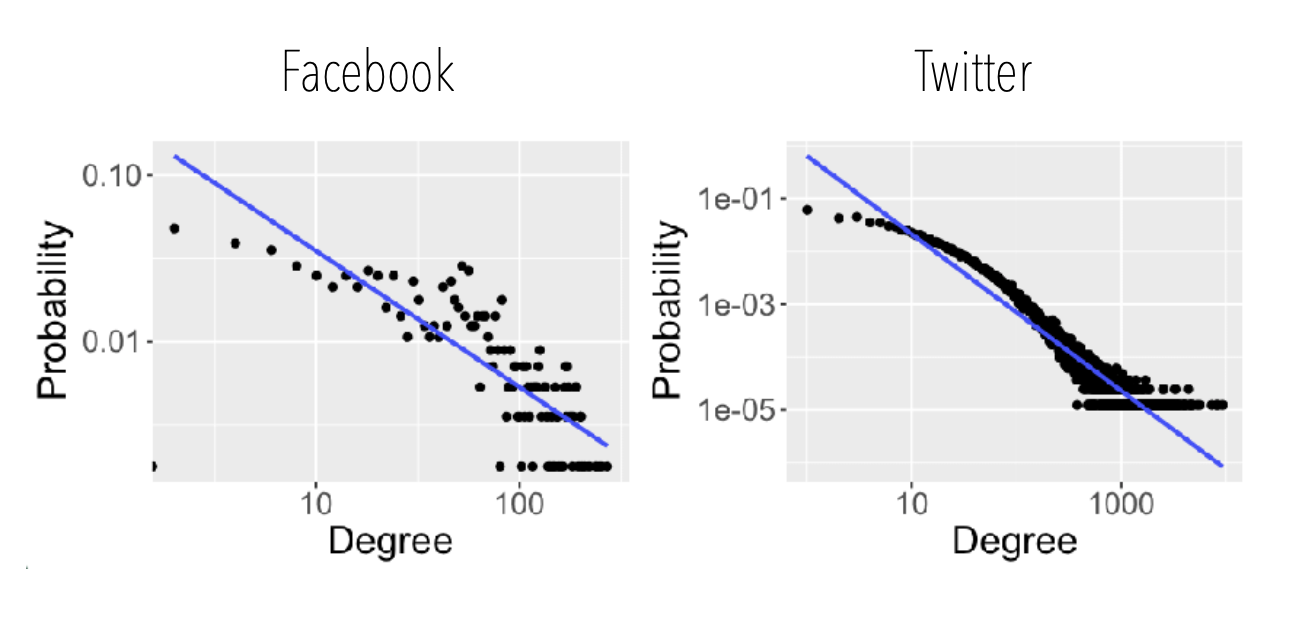
\includegraphics[width=0.8\textwidth]{../lessons/image/06/4.png}
\caption{\label{fig:06_3} Real network of Facebook and Twitter.}
\end{figure}

\subsection{Scale-free networks}

However, so far we have not discussed how real networks look like, in particular what is their degree distribution. In the last decades we started to have really complex and large networks, whose structure really differs from the structure we usually see for a random network. In Fig. \ref{fig:06_4}, as an example, we shown two real social networks we know pretty well: Facebook and Twitter. Note that both plots are in log-log scale. Generalizing, we can say that most of the real networks scales in the same way.\\ 
We now want to understand how the \textbf{degree distribution} looks like. Let us consider Fig. \ref{fig:06_4}: black dots follow the Poissonian distribution that we were mentioning before, while the squares follow a power-law \( P(k) \sim k^{- \gamma  } \), which is \textbf{heavy tailed distribution}, in the sense that possibility for large degrees is not null. One should note that the Poissonian distribution is not able to reproduce the heterogeneity we can see in the data, while the power-law is. Hence, in most contexts real networks are \textbf{highly heterogeneous} and degrees can span \textbf{several orders of magnitude}. In particular, the \( \gamma   \) coefficient of the power-law has an important role, since it represents the \textbf{slope} of the curve in log-log scale.\\
Since we observe similar structures for different scales, these networks are said to be \textbf{scale-free} networks. In most real networks $\gamma$ has small values, i.e. \( \gamma \le 3 \).


\begin{figure}[h!]
\centering
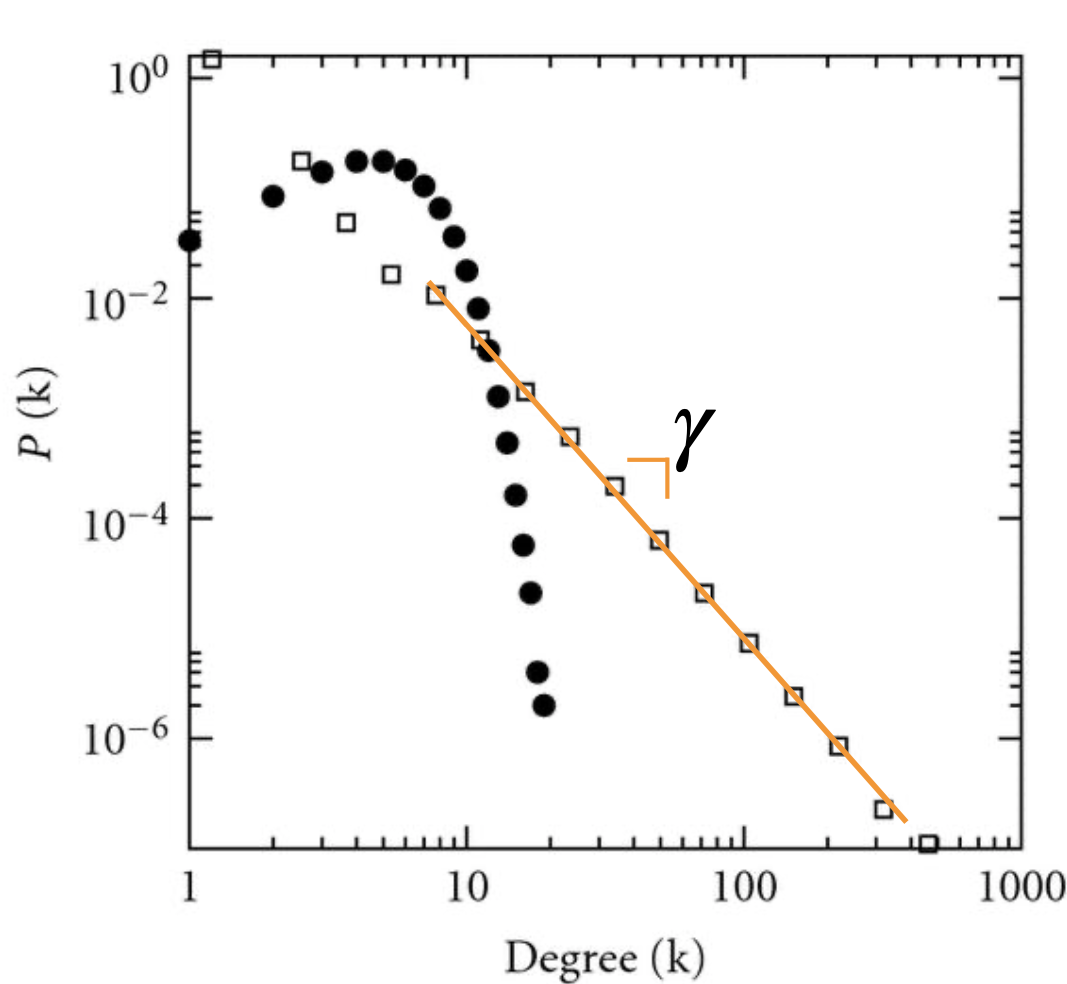
\includegraphics[width=0.7\textwidth]{../lessons/image/06/5.png}
\caption{\label{fig:06_4} Difference between random networks and scale-free networks.}
\end{figure}

\textbf{Heterogeneity} means that almost all nodes have a very low connectivity, way less than a random net. However, the probability of having very large degrees is not zero (\textbf{hubs}): even for relatively small networks we can observe large hubs. One should take into account that this is something really important for the spreading of diseases: thanks to these large hubs we can see shortcuts for spreading, or the so called \textbf{super-spreaders}.\\

We want now to study the \textbf{limiting cases} of these scale-free networks. For instance, we want to see how the \textbf{average degree} behaves, or prove that the \textbf{largest degree} scales with the size of the network. Let us consider the power-law:
\begin{equation}
  P(k) = C_0 k^{-\gamma } \qquad \text{with} \quad C_0 = (\gamma -1  ) k_{min}^{\gamma -1 }
\end{equation}
To understand how \( k_{max} \) scales with \( N \), we have to study the case where:
\begin{equation*}
  \int_{k_{max}}^{\infty } P(k) \dd[]{k}  = \frac{1}{N} \quad \rightarrow  \qty(\frac{k_{min}}{k_{max}})^{\gamma -1 } = N
\end{equation*}
Thus, when:
\begin{equation}
  k_{max} = k_{min} N^{\frac{1}{\gamma -1 }}
\end{equation}
Since in most of networks \( \gamma \sim 2-3  \), so it is easily to understand that $k_max$ scales \textbf{sub-linearly} with N, but still way faster than random graphs. This is valid for previous plots, such as in Fig. \ref{fig:06_3} as well.\\
Recalling the definition for the general \( n^{th} \) moment of a distribution: 
\begin{equation}
  \expval{k^n} = \int_{k_{min}}^{\infty } k^n P(k) \dd[]{k} = \int_{k_{min}}^{\infty }  C_0 k^{n- \gamma  }\dd[]{k}
\end{equation}
We note as it converges only if \( \gamma -1 > n  \). This gives an hint on how the \textbf{average degree} scales as the size of the network: a very important result. If instead we consider the variance \( \sigma ^2  = \expval{k^2} - \expval{k}^2  \), we it holds that:
\begin{itemize}
\item if \( \gamma <2  \), both \( \expval{k}  \) and \( \expval{k^2}  \) diverge with \( N \rightarrow  \infty  \);

\item if \( 2 < \gamma < 3  \), the average degree \( \expval{k}  \rightarrow c \) but \( \expval{k^2}  \rightarrow \infty \) as \( N \rightarrow  \infty  \), and \( \sigma ^2 \rightarrow \infty  \).
\end{itemize}
Remembering that most real networks have \( \gamma \le 3 \), hence the \textbf{variance of the degree also diverges}. The result is that we have extremely \textbf{heterogeneous networks} and not homogeneous ones. This is indeed coherent to our observations. 
It has indeed a very strong \textbf{implication}: all the models we have been using before, in which we assumed that \textbf{all the people} in the population were \textbf{equal}, does \textbf{not hold} anymore.

\subsection{Barabási-Albert Model}
So far we have discussed about scale-free networks, but actually we have not created a single one yet. Therefore, an \textbf{algorithm} to create such network we can rely on, is the \textbf{Barabasi-Albert model}. This topic is discussed in a paper that is the second, chronologically speaking, that gave birth to modern Network Science. \\
The \textbf{idea} behind this paper is extremely simple: once some real networks had been analyzed they assumed that the degree distribution \( P(K) \sim k^{-3} \), in order to create a model to reproduce the behaviors observed.\\
Moreover, their model was based on the concept of \textbf{growing} for random networks. We start with a small number of nodes, named \textbf{clique}, and, at each time-step, a new node enters the network and connects with pre-existing nodes but according to a \textbf{preferential attachment}. Therefore, at each step the network grows in size.\\
The principle on which \textbf{preferential attachment} is based on is a very simple concept: \textit{rich gets richer}. That is to say: the more connected a node is, the more likely it is for it to receive new links. The probability for a node $i$ to attract a new link at time $t$, is proportional to its degree $k_i$ at time $t$:
\begin{equation}
  \Pi (k_i) = \frac{k_i}{\sum_{j}^{} k_j }
\end{equation}
If we speak about \textbf{influencers}, having them a lot of followers, the probability for them to increase their connections is very high. Actually, this idea is not even new, and it is something already known. Indeed this model is just a modification of the \textit{Price model}: if we published a paper and more than someone has found it interesting, it will be more likely for it to receive much more attention in the future.\\
Specifically for this model, we are drawing links at random, according to some probability that indeed is not uniform. Let us briefly summarize the\textbf{main steps} of the algorithm:
\begin{itemize}
\item we start with a clique of \( m_0 \) nodes;
\item at each time step \( t \), we add a new node to the network;
\item we create $m$ (i.e. $m=2$) links between the new node and the existing ones according to the preferential attachment (remember to update the connection probability after each link);
\item repeat until the desired size $N$ is reached.
\end{itemize}
In particular, let us consider Fig. \ref{fig:06_5}. We start with a small number of nodes connected via some links. At the \textit{first time step} we add a new node, and then we need to draw connections to the other nodes. Let us assume that every time we add a node, we are adding two links. First, we need to compute the set of probabilities of connecting to each node and, at the first time-step, is equal for all the nodes. Then we pick up one node at random and we draw the link. The following step is to update the set probabilities for each node, according to their degree. We see that the node on the left has got an higher probability of getting new connections since the last node inserted has linked to it. Then, we iterate this procedure by introducing a new node and draw connections following the same procedure, until we end up with a total number of \( N \) nodes.

\begin{figure}[h!]
\begin{minipage}[c]{0.48\linewidth}
\centering
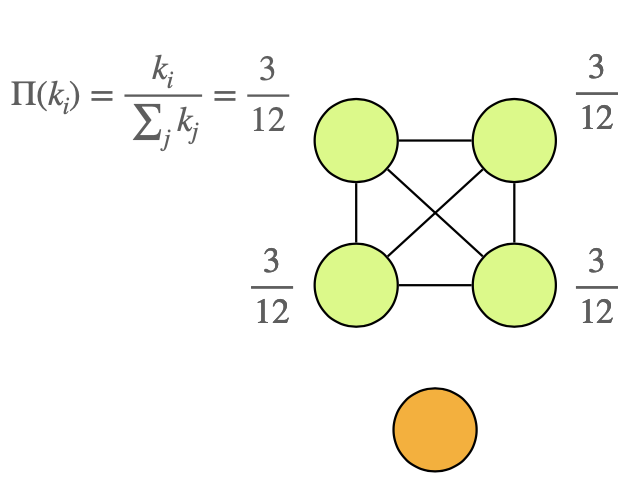
\includegraphics[width=0.8\textwidth]{../lessons/image/06/6.png}
\end{minipage}
\( \longrightarrow  \)
\begin{minipage}[]{0.48\linewidth}
\centering
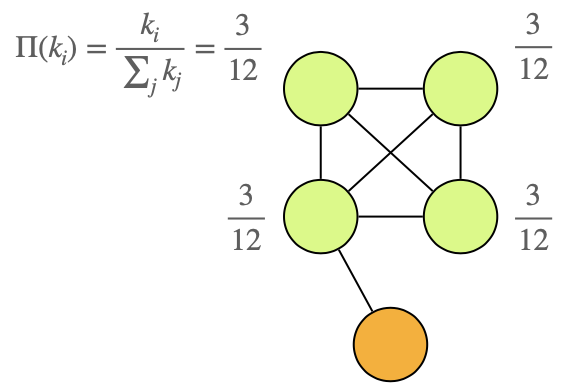
\includegraphics[width=0.8\textwidth]{../lessons/image/06/7.png}
\end{minipage}
\caption{\label{fig:06_5} Example of Barabási-Albert algorithm.}
\end{figure}

This algorithm is indeed able to create networks with some \textbf{interesting properties}. Indeed we can approximate the \textbf{degree distribution} as:
\begin{equation*}
  P(k) = \frac{2 m (m +1)}{k(k+1)(k+2)} \sim k^{-3}
\end{equation*}
where $m$ is the number of links we are adding at each step. Note that $m$ is a parameter that is related the minimal degree of the network. However, this approximation is valid for \textbf{large} \( k \).\\
An important result is that \( \gamma =3  \) and it is \textbf{independent} of \( m \) and \( m_0 \).\\
Hence, the \textbf{maximum degree} of the network scales as \( k_{max} \sim N^{1/2} \). Moreover, it holds that \( \expval{k} \rightarrow c \), but \( \expval{k^2} \rightarrow \infty   \) with \( N \), as we have seen before.
Finally, the \textbf{average length} of the network is:
\begin{equation*}
  \expval{l} \sim \frac{\ln (N)}{\ln (\ln (N))}
\end{equation*}
which tells us that the small-world property holds as well.










\chapter{Epidemic Spreading on Networks}

Now it is time to drop the assumption of the well-mixed population, and start taking into account \textbf{contact networks}. In other words we are considering that \textbf{individuals can be connected in different ways} one another.\\
The main idea is that:
\begin{itemize}
\item \textbf{all} individuals are \textbf{equivalent};
\item we remove the assumption that all individuals have the same number of contacts and we assume that each node \textbf{do not interact at random}. This reflects the reality, since we usually have more contacts with some people (friends, family, colleagues...) rather than others. The fact that we may have repeated contacts with someone else has strong effects on the dynamics: we are somehow constraining the way how the disease will spread.
\end{itemize}

\section{SIS model in a network}
Let us try to build a general model for a general network, without making any assumption on the latter. In order to do that, we start by introducing the equations of SIS model for a generic network.\\
The first step is to define a \textbf{binary variable} for each node \( i \): \( \sigma _i (t) \). This variable can only take two values:
\begin{itemize}
\item \( \sigma _i (t) = 0 \), if the individual is \textbf{susceptible};
\item \( \sigma _i (t) = 1 \), if the individual is \textbf{infected}.
\end{itemize}
As one can easily see, this variable describes the state of a generic $i$-th node at time $t$.\\
Defining another variable \( \rho (i,t) \):
\begin{equation*}
  \rho (i,t) \equiv \text{Prob} \qty[\sigma _i (t) = 1]
\end{equation*}
which represents the \textbf{probability} of that node \( i \) is infected at time \( t \).\\
Using this formalism, we can recall the general equation for the SIS in a network:
\begin{equation}
  \dv{}{t} \rho (i,t) = \overset{\text{Recovery}}{- \mu  \rho (i,t)} + \overset{\text{Infection}}{\beta \sum_{j}^{} A_{ij} \mathcolorbox{green!20}{\text{Prob} [\sigma _i (t) = 0, \sigma _j (t ) =1 ]   }}
\end{equation}
The most problematic part is to compute the two nodes infection probability (in green). Since we are in a network, the probability of being infected depends on my neighbours: the \( (i,j) \) infection probability depends on the status of all the other neighbors \( l \) of \( j \) and \( i \) and so forth.\\
Therefore we would have to follow the entire \textbf{chain of connections}, but this would turn out to be a problem: we cannot obtain a closed form for this expression, since it actually depends on the probabilities of all its neighbors. In turn, they would depend on their neighbors probability and so and so forth.\\
We want to stress one more time that if we want to predict what is going to happen in the system, we would need to consider the entire network and the time evolution for all the nodes. This approach however is \textbf{feasible} only for \textbf{small graphs} (i.e. 4/5 nodes) and \textbf{few compartments}.\\
This argument reminds us that we may need some sort of an \textbf{approximation}: indeed we need to \textbf{cut down} this \textbf{probability chain}. That is to say that, at some point, we require a closure of our equations, by the mean of approximation: we are not going to take into account the entire structure of the network. At some point we will take the \textbf{average}, and after that we will be able to solve the problem.\\
In physics this kind of arguments are called \textbf{mean-field approximations}. Since we are not able to solve many body problems, at a certain point we will consider a \textbf{random field} which \textbf{acts on the entire system} and we will consider its average effects on the system.\\
Tailoring this procedure to our specific problem, we are substituting in some way the probability \( \text{Prob} \qty[\sigma _i (t) = 0, \sigma _j (t ) =1 ]  \) with some average probability. Obviously, depending on the assumption we are making for this approximation, we will obtain different results.\\
There are actually many different types of approximations based on different features:
\begin{itemize}
\item \textbf{Network structure}:
    \begin{itemize}
    \item \textbf{Homogeneous} mean-field (all the nodes are equal);
    \item \textbf{Heterogeneous} mean-field;
    \end{itemize}
\item \textbf{Coarsening level}:
    \begin{itemize}
    \item \textbf{Degree-based} mean-field theories (DBMF) in which we assume that all the nodes of the same degree are equal;
    \item \textbf{Individual-based} mean-field theories (IBMF) in which we assume that all the nodes are different and that we will take individual connections between individuals;
    \end{itemize}
\item \textbf{Where to cut the chain}:
    \begin{itemize}
    \item \textbf{Individual} level;
    \item \textbf{Pair} approximations;
    \item \textbf{Triangles}, etc...;
    \end{itemize}
\end{itemize}


\subsection{Homogeneous Networks}
Let us start by taking the simplest approximation: we assume \textbf{homogeneous network}, \textbf{DBMF} and we cut the chain at an \textbf{individual} level.\\

It means that we are considering networks where \textbf{nodes degree} is \textbf{bounded}, hence:
\begin{itemize}
\item we have that \( k_i \simeq \expval{k}  \);
\item we have also that the standard deviation is bounded \( \frac{\sigma _k}{\expval{k} } = \sqrt{ \frac{1-p}{p(N-1)} } \overset{N \rightarrow \infty }{\longrightarrow} 0\).
\end{itemize}
All the \textbf{nodes} can \textbf{be assumed to be equal}, so their position on the network does not matter anymore. This implies the \textbf{spatial homogeneity} it holds that: \( \rho (i,t) \equiv \rho (t) \).\\
In addition, cutting at the individual level means that the two terms of the \textbf{joint probability} of one being infected and the other one being susceptible \( \text{Prob} [\sigma _i (t) = 0, \sigma _j (t ) =1 ] \) are \textbf{statistically independent}. This implies that the joint probability can be factorized as follows:
\begin{equation*}
  \text{Prob} [\sigma _i (t) = 0, \sigma _j (t ) =1 ] \qquad \rightarrow \qquad \text{Prob} [\sigma _i (t) = 0] \cdot \text{Prob} [\sigma _j (t ) =1 ]
\end{equation*}
But now we recall that:
\begin{equation*}
  \rho (t) = \text{Prob} [\sigma (t)=1]
\end{equation*}
is the density of infected at time \( t \).
Hence, putting everything together, we derive the equation:
\begin{equation*}
  \dv{\rho }{t} = - \mu \rho  + \beta \sum_{j}^{} A_{ij} (1- \rho ) \rho \qquad \rightarrow \qquad
   \dv{\rho }{t} = - \mu \rho  + \beta (1- \rho ) \rho \sum_{j}^{} A_{ij}
\end{equation*}
Actually, this last term is the degree of the network:
\begin{equation}
  \sum_{j}^{} A_{ij} = k_i \simeq \expval{k}
\end{equation}
and by replacing it, we can obtain the same expression that we derived before for SIS model in a well-mixed population:
\begin{equation}
  \dv{\rho }{t} = \beta \expval{k} (1- \rho ) \rho - \mu \rho
\end{equation}
This is a very important result.\\
One should keep in mind that now we are considering all the \textbf{nodes statistically independent} and we are back again to exactly the same result of well-mixed population. The only \textbf{difference} is that when we were considering well-mixed population, we assumed that the \textbf{probabilities} where \emph{exactly} \textbf{statistically independent}. Now, this is just an \textbf{approximation}.\\
Obviously, all the results derived for SIS model in well-mixed populations are still valid, for instance the epidemic threshold.

\begin{remark}
Let us recap what we have seen at the end of this lecture.\\
We moved from well-mixed populations to contact networks, so we added more complexity in order to make the model is more realistic. We also derived the equations for SIS dynamics on a generic network and then considered its adjacency matrix. Since for us was impossible to write down a closed equation for this model, given the expression for the infection joint probability that involves two nodes, we were not able to compute exactly the probability for a single node of being infected ($\rho_i$). It would take into account the probability of three nodes \( i j k \) at the same time. This is actually unfeasible for all the models and all the possible graphs: it has been done in the literature up to only 4/5 nodes. Hence we end to somehow approximate this probability, in order to cut this infinite chain to a certain value. This is exactly why we introduce mean-field approximation: in this way we take into account the effects of all terms on a specific quantity, not individually, but on average therefore reducing the complexity of our problem. We are switching from a many body problem to a one body problem.\\
The simplest approximation we have seen is the one of homogeneous network in which all the nodes are equal, used on SIS model. According to this argument, for each node there is the same probability of getting infected, so we can approximate the probabilities to be statistically independent. After, we derived all the equations. Their solutions were the same as the ones we had found for well-mixed population. However, in that case the solutions found were \textit{exact}, while now are the result of an approximation.
\end{remark}





\end{document}
